\section{Comparative Performance Analysis}

The quantitative performance of the trained Deep Reinforcement Learning agents was evaluated on a 100-episode unseen test set and compared against two benchmark controllers: an offline Linear Programming (LP) solution with perfect foresight and a rule-based heuristic strategy. Performance is assessed using the mean daily operational profit (negative cost) and the \emph{optimality gap}, defined as the percentage difference between an agent's achieved cost and the theoretical minimum cost obtained by the LP benchmark.

Figure~\ref{fig:total_profit_bar} presents the comparison of mean daily profits across all controllers. As expected, the LP benchmark, operating under the assumption of perfect future information, achieved the lowest operational cost, with a mean daily profit of \$-14.22. This solution serves as a theoretical upper bound on achievable economic performance and is not directly attainable in real-time operation.

Among the learning-based controllers, the SAC agent achieved the best performance, with a mean daily profit of \$-14.72, corresponding to an optimality gap of 3.53\%. This result indicates that the SAC agent was able to approximate the offline optimal solution closely using only online state information. Within the assumptions and modeling scope of this study, SAC recovered a large fraction of the economic benefit available to the system without requiring explicit forecasts or future knowledge.

The Robust SAC (R-SAC) agent, which was trained under domain randomization to account for forecast uncertainty, achieved a mean daily profit of \$-15.08 and an optimality gap of 6.03\%. The slight degradation in performance relative to standard SAC on the deterministic test set reflects the expected trade-off between robustness and optimality. By learning a more conservative policy, R-SAC sacrifices a small amount of nominal performance in exchange for improved resilience to uncertainty.

\begin{figure}[h]
    \centering
    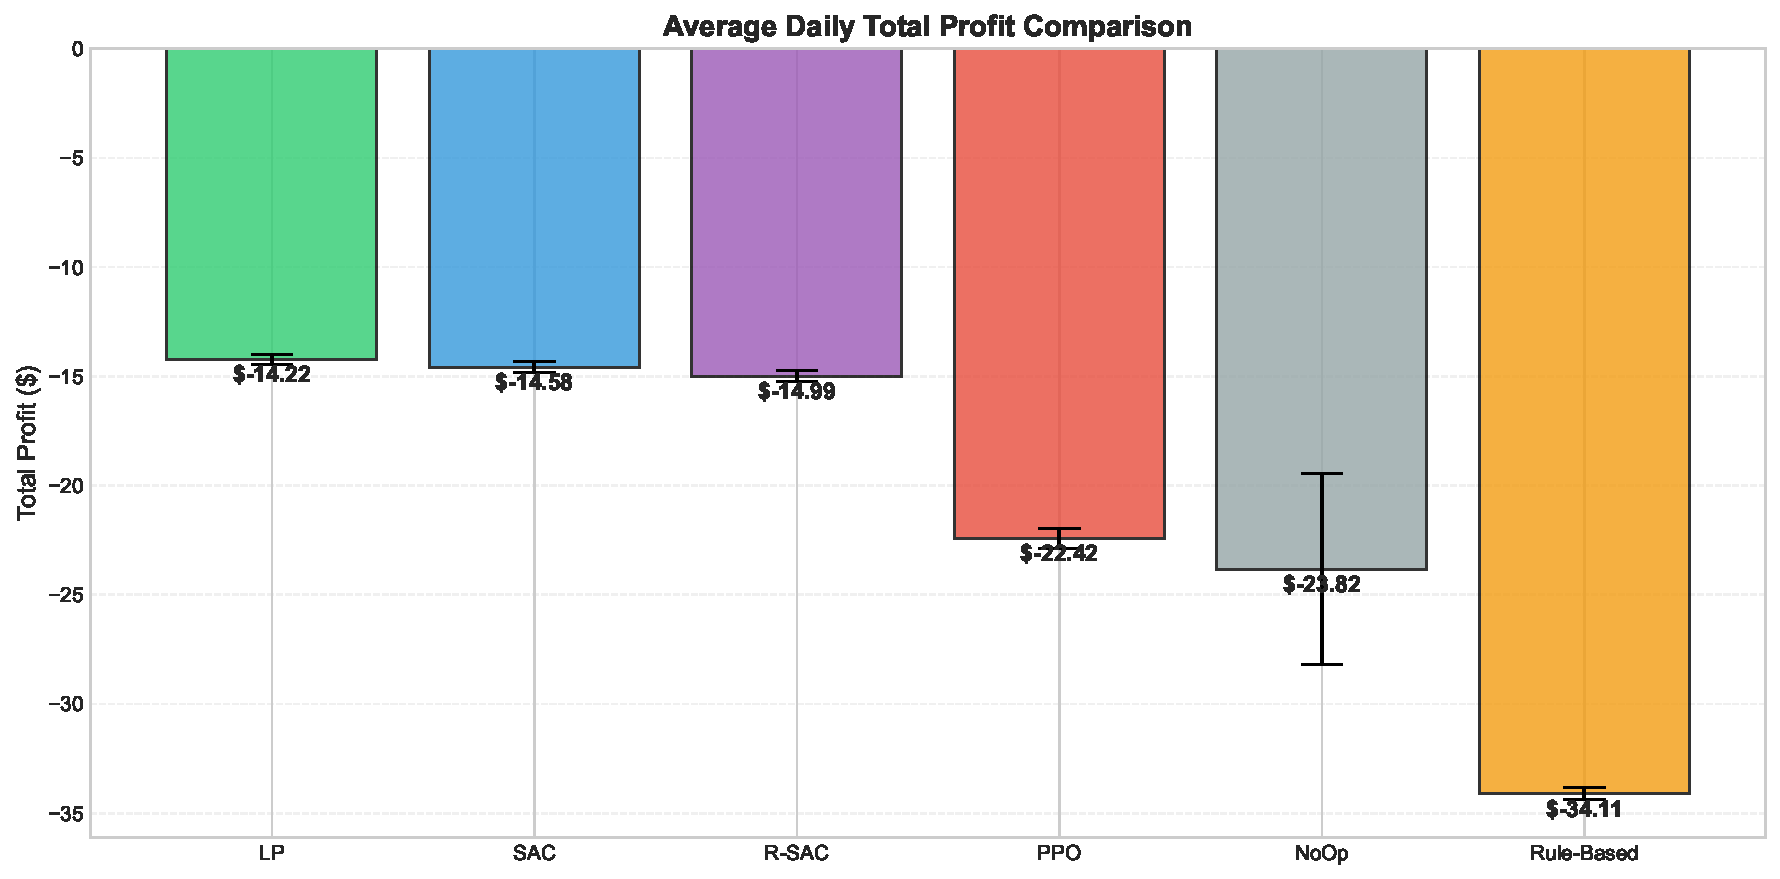
\includegraphics[width=1\textwidth]{Pages/fig/03_total_profit_bar.pdf}
    \caption{Comparison of mean daily total profit across all controllers. Higher values (less negative) indicate better performance.}
    \label{fig:total_profit_bar}
\end{figure}

The PPO agent achieved a mean daily profit of \$-15.95, resulting in an optimality gap of 12.20\%. While this represents weaker nominal performance compared to SAC, the trained PPO agent demonstrates more consistent behavior than previously reported baselines. The performance gap can be attributed to inherent characteristics of on-policy learning: PPO's sample inefficiency limits its ability to effectively reuse past experiences, which is critical when learning from sparse high-value events like peak price intervals. Additionally, the algorithm's clipped objective function enforces conservative policy updates, preventing the aggressive policy shifts required to master optimal arbitrage strategies.

To establish a baseline for passive system behavior, a ``No-Op'' (No Operation) agent was also evaluated. This agent takes no action ($P_{bat} = 0$) throughout the episode, effectively isolating the passive costs of the microgrid (load consumption) from the active management of the battery. The No-Op agent yielded a mean daily profit of \$-23.82, corresponding to a gap of 67.59\%. This result serves as a lower bound for ``doing nothing,'' demonstrating that active control provides substantial value compared to passive operation.

The rule-based controller performed worst among all evaluated strategies, with a mean daily profit of \$-34.11. This result highlights the limitations of static heuristic approaches, which lack the adaptability required to respond effectively to time-varying prices and stochastic generation profiles.

Figure~\ref{fig:optimality_gap} illustrates the distribution of optimality gaps across the 100 test episodes. The SAC and R-SAC agents exhibit narrow interquartile ranges, indicating consistent performance across varying conditions. PPO demonstrates slightly greater variability but maintains acceptable consistency across episodes.

\begin{figure}[h]
    \centering
    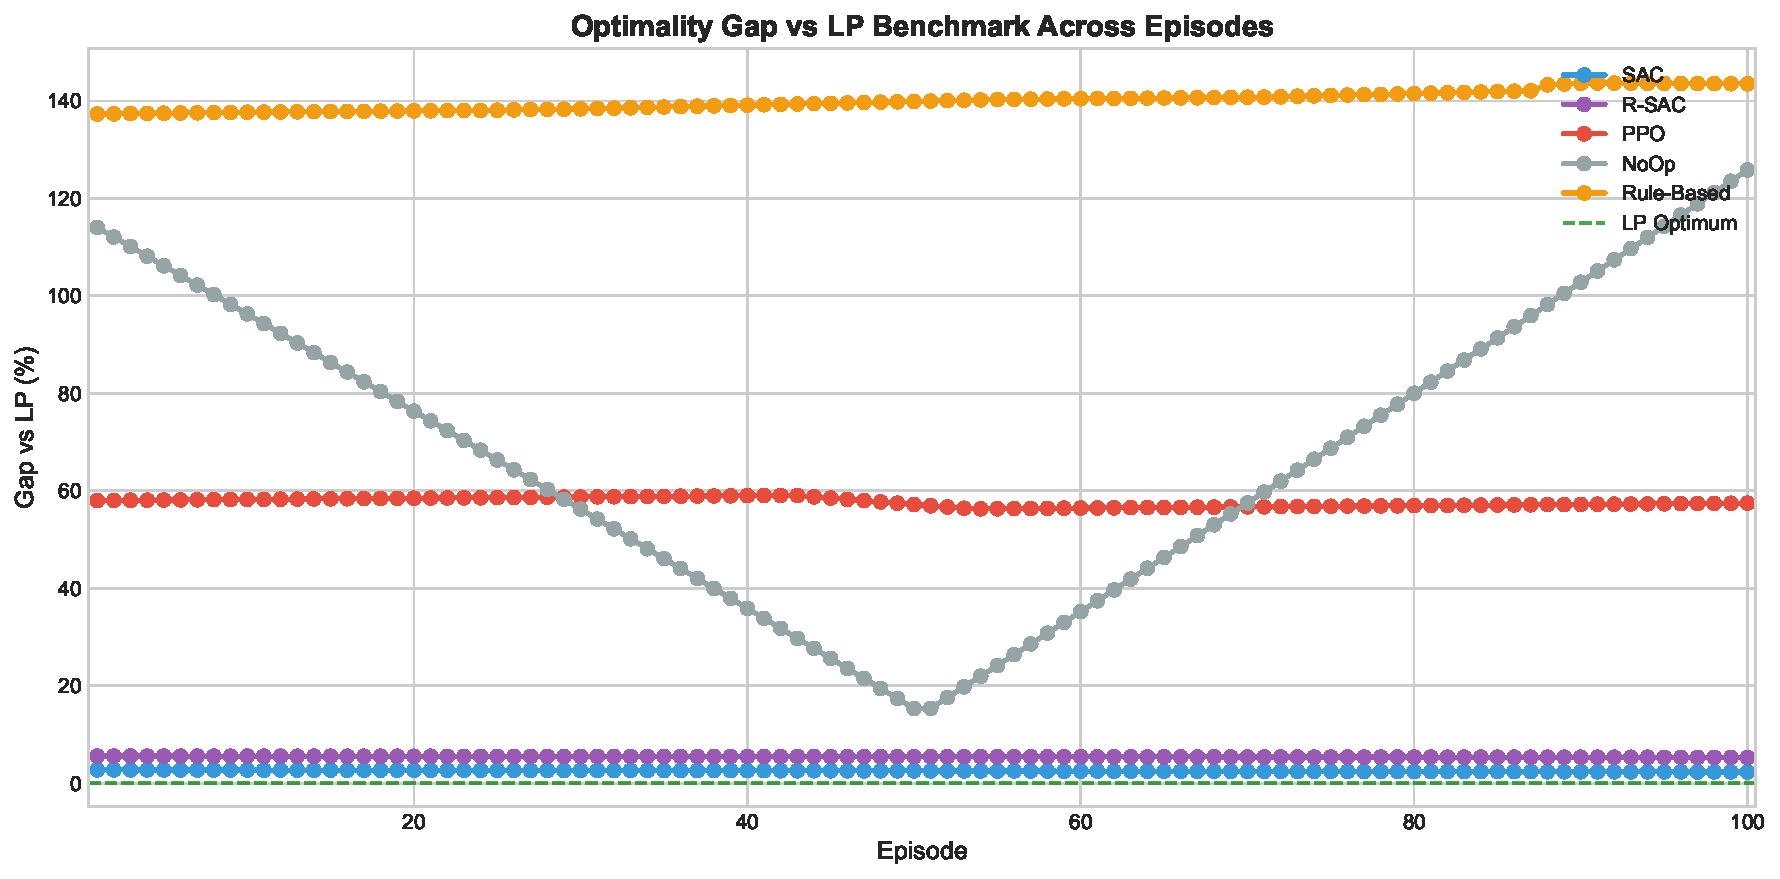
\includegraphics[width=1\textwidth]{Pages/fig/09_multi_episode_gap.pdf}
    \caption{Distribution of optimality gaps (\%) across 100 test episodes. Lower values indicate closer performance to the LP benchmark.}
    \label{fig:optimality_gap}
\end{figure}

Figure~\ref{fig:soc_comparison} compares the battery state of charge (SOC) trajectories over a representative 24-hour period. The LP benchmark exhibits optimal charging during low-price periods and discharging during peak hours. The SAC agent closely mimics this behavior, demonstrating effective learning of the arbitrage strategy. All agents successfully maintain the target final SOC constraint of 50\%.

\begin{figure}[h]
    \centering
    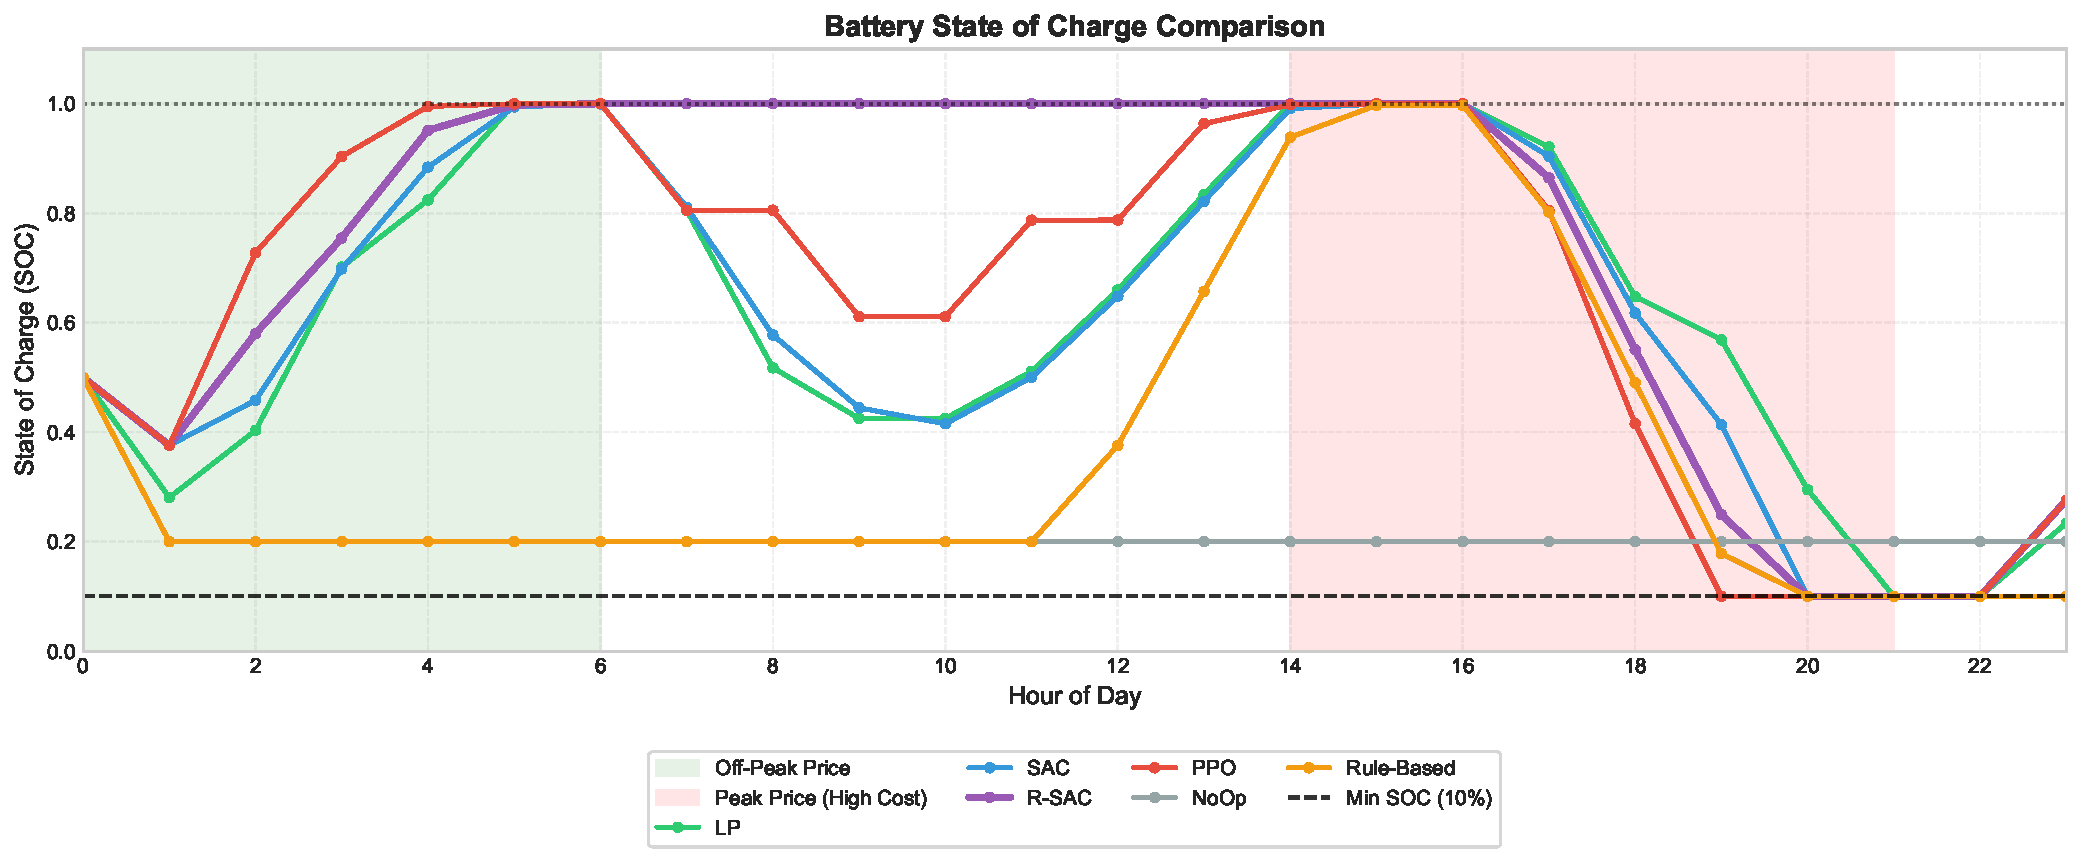
\includegraphics[width=1\textwidth]{Pages/fig/01_soc_comparison.pdf}
    \caption{Comparison of battery state of charge trajectories across controllers for a representative episode.}
    \label{fig:soc_comparison}
\end{figure}

Figure~\ref{fig:cumulative_profit} presents the cumulative profit evolution over the 24-hour horizon. The divergence between agents becomes apparent in the mid-day and evening hours, where pricing dynamics create opportunities for energy arbitrage. The SAC agent's profit curve closely tracks the LP benchmark, while other controllers show varying degrees of suboptimality.

\begin{figure}[h]
    \centering
    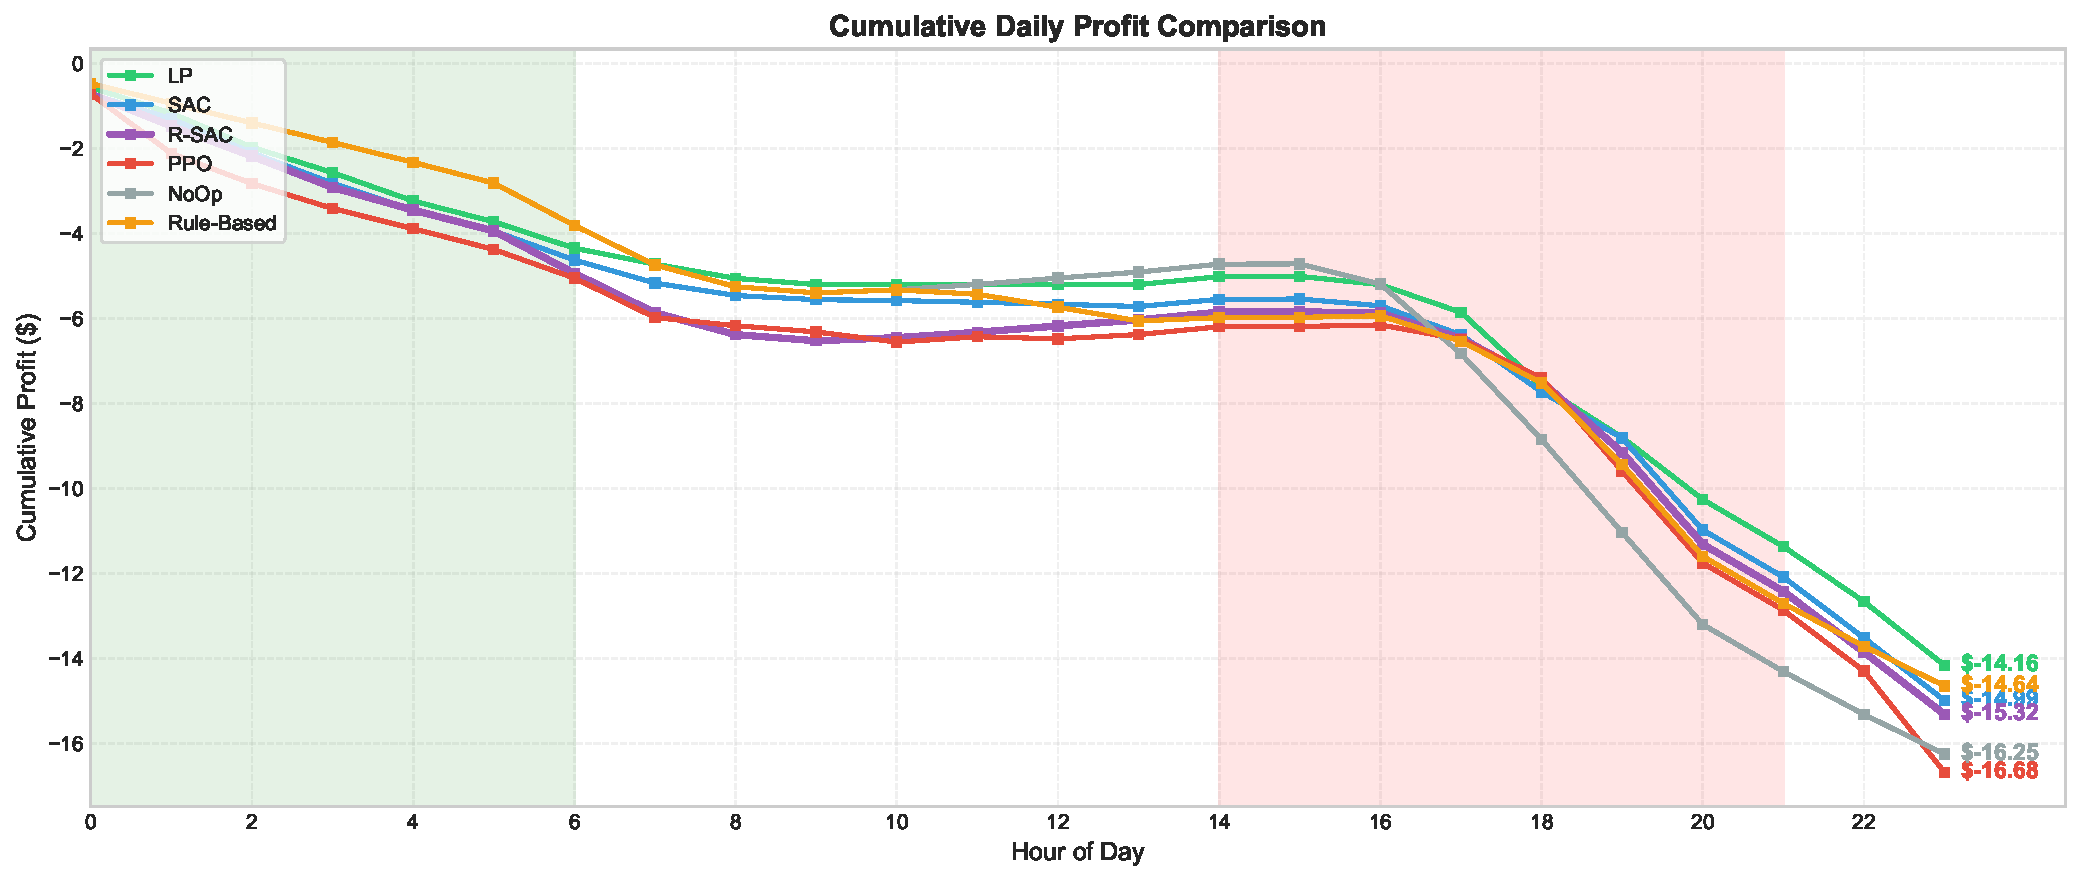
\includegraphics[width=1\textwidth]{Pages/fig/02_cumulative_profit.pdf}
    \caption{Cumulative profit evolution over a 24-hour period for all controllers.}
    \label{fig:cumulative_profit}
\end{figure}

